\documentclass[twoside]{article}
\input{ISC18-english.sty}
%%%%%%%%%%%%%%%%%%%%%%%%%%%%  Make sure to compile twice for proper cross-references. %%%%%%%%%%%%%%%%%%%%%%%
%%%%%%% For proper display of references, compile the document twice. %%%%%%%%%%%%%%%%%%%%% 
%%%%%%%%%%%%%%% If using TeX Live, compile using pdflatex command %%%%%%%%%%%%%%%%%%%%%%%
\begin{document}
\thispagestyle{empty}
%%%%%%%%%%%%%%%%% Article title header  %%%%%%%%%%%%%%%%%%%%
\fancyhead[LE]{Optimal lot reinspection  based on truncated life test...}
%%%%%%%%%%%%%%%%% Article authors header   %%%%%%%%%%%%%%%%%%%%
\fancyhead[RO]{Naghizadeh Qomi}
\begin{center}
{
\includegraphics [height=25mm, width=150.3mm] {Images/isc18E}} \\
\vspace*{-1.8cm}
%\begin{center}
%\color{blue} 
%{\hspace{0.1cm}\rule{\textwidth}{1mm}}\\
%\end{center}
\vspace*{4cm}
%%%%%%%%%%%%%%%%% Article title  %%%%%%%%%%%%%%%%%%%%
{\Large \bf Optimal lot reinspection  based on truncated life test for logistic Rayleigh distribution}\\
%%%%%%%%%%%%%%%%% Article authors and affiliations %%%%%%%%%%%%%%%%%%%%
{\bf
Mehran Naghizadeh Qomi\footnote[1]{{\bf Corresponding Author:} {\tt m.naghizadeh@umz.ac.ir }} \\
Department of Statistics, University of Mazandaran, Babolsar, Iran}
\end{center}
\rule{\textwidth}{0.2mm}\\
%%%%%%%%%%%%%%%%% Article abstract  %%%%%%%%%%%%%%%%%%%%
\noindent{\bf Abstract:}\\
Single sampling scheme is a conventional method for evaluating the equality of lots of products. Repetitive sampling plans are introduced in order to reduce the size of samples drawn from the lot. The product lifetime follows the logistic Rayleigh distribution. Best repetitive sampling plans are determined by minimizing the sampling effort using integer nonlinear programming. In terms of average sample number, optimal repetitive sampling plans outperform single sampling plans.  A practical application is included for illustrative purposes.\\
\noindent{\bf Keywords:} 
Quality control, Repetitive sampling plans, Average sample number, Producer and Consumer risks. \\
\noindent{\bf Mathematics Subject Classification (2010):} $\rm 62N05$, $\rm 62P30$. \\
\hspace{1cm}\rule{\textwidth}{0.2mm}\\
%%%%%%%%%%%%%%
\section{Introduction}
Acceptance sampling plans are usually designed to decide the acceptability of submitted lots. In these plans, the lots of the product are tested using inspection schemes to determine if they are accepted or rejected based on random samples selected from them. 
Designing of inspection plans must provide appropriate protections to both producers and consumers while minimizing the sampling inspection effort to find the best plan. The constrained optimization problems can be solved to obtain the best inspection plan.
Methods to determine sampling plans have been widely studied. Among others, we can cite    \cite{NF2024},  \cite{NPGF2025} and \cite{NA2026}.


Single sampling is the classical and most frequently used inspection scheme applied in practice. In this scheme, the lot is accepted if the number of failed products (defectives) in the selected sample is sufficiently low. However, in many cases, a single inspection can lead to occasional incorrect decisions about entire lots of products. In such situations, lot reinspection may be desirable to ensure the correctness of the decision. 
This type of plans are often more effective in reducing sample sizes. For example, repetitive sampling  is an inspection method in which the acceptance and rejection of the lot is based on the repeated sample results of the same lot. 
The repetitive  sampling plan (\textit{RSP}) in lot inspection  was introduced by \cite{Sherman}
and has been thoroughly examined br researchers. See \cite{Jeya2025}, \cite{NM2025} and \cite{NFC2026}.


\cite{Cha} introduced the logistic-Rayleigh (\textit{LR}) distribution as a suitable model for  real life applications and survival analysis. During the literature exploration, it was observed a lack of initiative in establishing \textit{RSP}s for \textit{LR} distribuion. In this paper, we employ the  repetitive methodology to design optimal time-censored (or type-I censored) reliability sampling plans with limited producer's and consumer's risks when the lifetime variable follows \textit{LR}  distribution.


The remainder of this work is structured as follows.
A single sampling plan (\textit{SSP}) based on  \textit{LR} distribution is presented in Section 2.
In Section 3, we describe the   \textit{RSP} methodology for the assumed probability distribution along with their mathematical formulation.
A discriptive and comparative analysis of the proposed inspection scheme is provided in Section 4.
 Section 5 uses a real data set to illustrate the proposed plan in real-life situations.
Section 6 concludes the paper with a summary of findings and relevant considerations.



\section{\textit{LR} single sampling plans}
Suppose that a reliability engineer wants to judge the acceptability of a large lot of products. Assume that the random variable $T$ represents the product lifetime and also that the distribution of $T$ is \textit{LR} with the shape and scale parameters $\delta>0$ and $\theta>0$, repectively, i.e., $T\sim LR(\delta,\theta)$. 
The probability density function (pdf) and the corresponding cummulative distribution function (cdf) of $T$ are given respectively by 
\begin{eqnarray}\label{pdfcdf}
f(t;\delta,\theta)=\frac{\delta\theta te^{\theta t^2/2}[e^{\theta t^2/2}-1]^{\delta-1}}{(1+[e^{\theta t^2/2}-1]^{\delta})^{2}}~~\textrm{and}
~~F(t;\delta,\theta)=1-\frac{1}{1+[e^{\theta t^2/2}-1]^{\delta}},~~t>0.
\end{eqnarray}
The pdf of the \textit{LR}  distribution is right-skewed and then  the median quality characteristic can be  used to indicate the
quality of product. The median of $T$ is given by $\mathcal{M}=[(2\log 2)/\theta]^{\frac{1}{2}}$.

Assume that  $p$ denotes the true proportion nonconforming. When the lot size is large, 	the number $\mathcal{D}$ of defective units follows approximately a binomial distribution, that is, $\mathcal{D}\sim Bin(n,p)$.
%
An \textit{SSP} would be characterized by a pair $\mathcal{P}_1=(n,c)$ and the decision process associated with the inspection scheme $\mathcal{P}_1$ can be stated as follows: {\it Step 1:} Select $n$ units at random from the submitted lot and count the number $\mathcal{D}$ of defective units. \textit{Step 2:} Accept the lot if $\mathcal{D}\leq c$, where  $c$ is the so-called acceptance number and reject the lot otherwise.
%
The operating characteristic  (\textit{OC}) function which is the lot acceptance probability is given by
\begin{eqnarray}\label{LS}
\mathcal{L}_1(p)\equiv \mathcal{L}_1(p,n,c)=P(\mathcal{D}\leq c|p)=\sum_{i=0}^c {n \choose i} p^i(1-p)^{n-i},~~0<p<1.
\end{eqnarray}






\section{ Optimal \textit{LR} repetitive plans}
In a standard \textit{RSP}, the submitted lot is accepted if the number $\mathcal{D}$ of defective items in the chosen sample is small and rejected if it is large. Otherwise, the analyst has to repeat indefinitely the above process until a final decision is made. 
The procedure of a standard \textit{RSP} can be described as follows: Step1: Select a sample of size $n$ from the lot and put it on test for a pre-determined  time $t$.
Step 2: Accept the lot  If $\mathcal{D}\leq c_1$ and reject if $\mathcal{D}>c_2$, where $c_2\geq c_1$.
Step 3: If $\mathcal{D}\in(c_1,c_2]$, then go to Step 1 and repeat the decision process with a new sample.
%
%
The proposed  \textit{RSP}   is characterized by $\mathcal{P}_2=(c_1, c_2, n)$. If $c_1=c_2$, this plan reduces to \textit{SSP}.
%

The \textit{OC} function associated with $\mathcal{P}_2=(c_1, c_2, n)$ is defined as $\mathcal{L}_2(p)\equiv \mathcal{L}_2(p,n,c_1,c_2)$ which is given by
\begin{eqnarray}\label {oc}
\mathcal{L}_2(p)=\mathcal{L}_1(p,n,c_1)\sum_{j=1}^{\infty}\{\mathcal{L}_1(p,n,c_2)-\mathcal{L}_1(p,n,c_1)\}^j=\frac{\mathcal{L}_1(p,n,c_1)}{\mathcal{L}_1(p,n,c_1)+1-\mathcal{L}_1(p,n,c_2)}.
\end{eqnarray}
%
Let $\mathcal{M}$ be the true median lifetime of products and $\mathcal{M}_0$ is the minimal median lifetime that is acceptable to the consumer and producer. The quality level of a product  can be expressed as $r=\mathcal{M}/\mathcal{M}_0$.  The  termination time $t$ can be determined as a multiple of $\mathcal{M}_0$, that is  $t=d_0\mathcal{M}_0$, where $d_0$ is the termination ratio.
Moreover, the failure probability or proportion defective before time $t$ is $p\equiv p(\delta,\theta,r)$ which can be obtained as
$p=1-\frac{1}{1+[\exp\{{\frac{d_0^2\log 2}{r^2}}\}-1]^{\delta}}$.
%
%

Assume that $p_1$ and $p_2$ are the rejectable and acceptable   defective rates associated with the  consumer and producer, respectively. 
The   consumer and producer risks  are defined  as  $\sup_{p\geq p_1}\{\mathcal{L}_2(p)\}$ and $\sup_{p\leq p_2}\{1-\mathcal{L}_2(p)\}$, respectively.
Since $\mathcal{L}(p)$ is a decreasing function of $p$, then the consumer and producer risks are given by 
  $\mathcal{L}_2(p_1)$ and  $1-\mathcal{L}_2(p_2)$.
%%
%%
%%, 
 
Let $r_1$ and $r_2$ be the ratio of quality level corresponding to the consumer and producer, respectively.
 The consumer demands that
the lot acceptance probability should be smaller than the specified consumer's risk $\beta$ at a lower
quality level ($r_1=1$), whereas the producer requires that the lot rejection probability
should be smaller than the specified producer’s risk $\alpha$ at a higher quality level ($r_2>1$). 
%
%
%
  The inspection cost of $\mathcal{P}_2=(c_1,c_2,n)$ is measured by its average sample number (\textit{ASN}).  The \textit{ASN} at $p\in(0,1)$ is denoted by   $ASN(p)\equiv ASN(p,n,c_1,c_2)$ and it is defined by
\begin{eqnarray}\label{asn}
	ASN(p)=n\sum_{j=0}^{\infty}\{\mathcal{L}_1(p,n,c_2)-\mathcal{L}_1(p,n,c_1)\}^j=
\frac{n}{\mathcal{L}_1(p,n,c_1)+1-\mathcal{L}_1(p,n,c_2)}
\end{eqnarray}
Evidently, $ASN(p,n,c_1,c_1)\equiv n$, i.e., the \textit{RSP}  reduces to the \textit{SSP}. 
We are interested to obtain the optimal repetitive plans  $\mathcal{P}^{\star}_2=(c_1^{\star},c_2^{\star},n^{\star})$  that satisfies the nonlinear inequality constraints
$1-\mathcal{L}_2(p_2)\leq \alpha$ and $\mathcal{L}_2(p_1)\leq \beta$.
%
The constrained optimization problem is an integer nonlinear programming problem, which can be stated as follows:
%%%
%%%
%
\begin{equation}
\label{optim}
\begin{array}{lllll}
\text{Minimize} & ASN(p_1)  \\
\text{Subject to} & \mathcal{L}_2(p_1,n,c_1,c_2)\leq \beta,\\
                           &  \mathcal{L}_2(p_2,n,c_1,c_2)\geq 1-\alpha,\\
                           &0\leq c_1\leq c_2<n,                        
\end{array}
\end{equation}
where $n\in\mathbb{N}=\{1,2,...\}$ and $c_1,c_2\in\mathbb{N}_0=\mathbb{N}\cup\{0\}$.
 A step-by-step iterative method  to find the $ASN(p_1)$-optimal \textit{RSP} can be summarized as follows:
Step 1:~Set the value of parameter $\delta$, producer's and consumer's risks $(\alpha,\beta)$ and the termination ratio $d_0$.
Step 2: Set the initial values of plan parameters $n=1$, $c_1=0$ and $c_2=c_1+1$.
Step 3: Compute the probabilities $\mathcal{L}_2(p_1,n,c_1,c_2)$ and $\mathcal{L}_2(p_2,n,c_1,c_2)$ using equation (\ref{oc}) and $ASN(p_1)$ using equation (\ref{asn}). Then, check the inequalities $\mathcal{L}_2(p_1,n,c_1,c_2)\leq \beta$ and $\mathcal{L}_2(p_2,n,c_1,c_2)\geq 1-\alpha$.
Step 4: Obtain the different feasible plans $(n, c_1, c_2)$ verifying the above inequalities. From the feasible solutions, find the best plans $(n^{\star}, c_1^{\star}, c_2^{\star})$ that minimize the $ASN(p_1)$.
%%
%%
%%


\section{Descriptive and comparative analysis}
The behavior of the proposed \textit{RSPs} is analyzed in this section. 
%
The ASN-optimal repetitive LR plans  $(c_1^{\star},c_2^{\star},n^{\star})$ are presented in   Tables \ref{tab01} and \ref{tab02}   for $\alpha=0.01$, $\beta=0.05,0.10$, $r_1=1$, $r_2=2,3,4,5$, $d_0=0.5,1$ when $\delta=1$ and $\delta=2$, respectively.
%
From  Tables \ref{tab01}-\ref{tab02}, it can be observed that when considering the same values of $\delta$ and $r_2$, as the value of $d_0$ increases from 0.5 to 1.0, it becomes evident that there is a decrease in the magnitude of $n^{\star}$ and $ASN^{\star}$.  The optimal sample size $n^{\star}$ and value $ASN^{\star}$ generally becomes smaller when    $\beta$ increases. Moreover,  $ASN^{\star}$ value tends to decrease as  quality level $r_2$ increases. 



We then analyzed how the proposed RSP outperforms the SSP based on LR distribution. 	The minimum \textit{ASN} of the proposed  \textit{RSP} and the corresponding optimal sample size of \textit{SSP} are plotted in Figure \ref{fig1}  for $d_0=0.5,1.0$, $\alpha=0.01, \beta=0.05$ and $\delta=1$.  It is clearly evident that the proposed plan performs better than the $\it SSP$, in terms of \textit{ASN}.
%%
%%
%%%%
%%%%%
\begin{table} 
\tiny
 \centering
 \caption{\small Optimal \textit{RSPs} $(c_1^{\star},c_2^{\star},n^{\star})$ for selected values of $\beta, r_2$ and $d_0$ when $\alpha=0.01$ and $\delta=1$. }\label{tab01}
 \resizebox{\textwidth}{!}
 {
\begin{tabular}{cccccccccccccccc}
\hline
                &&            &&&    \multicolumn{4}{c}{$d_0=0.5$}  &&&&    \multicolumn{4}{c}{$d_0=1$}        \\
                       \cline{6-9}    \cline{13-16}    \vspace{2mm}
 $\beta$    && $r_2$  &&& $c_1^{\star}$ &  $c_2^{\star}$  & $n^{\star}$  &  $ASN^{\star}$ &&&&  $c_1^{\star}$  &  $c_2^{\star}$  & $n^{\star}$  &  $ASN^{\star}$ \\
\hline
 0.05    && 2  &&&    2   &   5  &   41& 59.8627  &&&&  2    & 5  &  12 & 18.9849\\
           && 3   &&&   0   &   2  &   20  &29.8870   &&&& 1  &   3  &   9 & 11.7551\\
           && 4   &&&   0   &   2  &   20  &29.8870   &&&& 0  &   2  &   6 &  8.9302\\
           && 5  &&&    0  &    1  &   19  &21.9298   &&&& 0  &   1  &   5   &5.9259\\
   \rule{0mm}{4mm} 
 0.10  && 2   &&&   1  &    4   &  28  &54.2724   &&&& 2   &  5   & 12  &18.9849\\
         && 3   &&&   0   &   2  &   17  &29.5615   &&&& 0   &  2   &  5  & 9.4118\\
         && 4   &&&   1  &    2  &   25  &29.1073   &&&& 1   &  2   &  7  & 8.3738\\
         && 5   &&&   0  &    1  &   15  &19.0100   &&&& 0   &  1   &  4  & 5.3333\\
\hline
 \end{tabular}}
 \end{table}
%%
%%
%%
\begin{table} 
\tiny
 \centering
 \caption{\small Optimal \textit{RSPs} $(c_1^{\star},c_2^{\star},n^{\star})$ for selected values of $\beta, r_2$ and $d_0$ when $\alpha=0.01$ and $\delta=2$. }\label{tab02}
 \resizebox{\textwidth}{!}
 {
\begin{tabular}{cccccccccccccccc}
\hline
                &&            &&&    \multicolumn{4}{c}{$d_0=0.5$}  &&&&    \multicolumn{4}{c}{$d_0=1$}        \\
                       \cline{6-9}    \cline{13-16}    \vspace{2mm}
 $\beta$    && $r_2$  &&& $c_1^{\star}$ &  $c_2^{\star}$  & $n^{\star}$  &  $ASN^{\star}$ &&&&  $c_1^{\star}$  &  $c_2^{\star}$  & $n^{\star}$  &  $ASN^{\star}$ \\
\hline
 0.05  && 2   &&&   0  &    2  &   97& 140.8509   &&&&  0  &  2 &   6 &8.9302\\
         && 3   &&&   0   &   1  &   90& 104.1581    &&&& 0 &   1 &   5 &5.9259\\
         && 4   &&&   0   &   1  &   90& 104.1581   &&&&  0  &  0 &   5& 5.0000\\
         && 5  &&&    0   &   0  &   86&  86.0000   &&&&  0  &  0 &   5 &5.0000\\
   \rule{0mm}{4mm} 
 0.10   && 2  &&&     0 &     2&     81& 136.8967  &&&&   0   & 1 &   4 &5.3333\\
         && 3  &&&     0   &   1  &   72 & 90.5450   &&&&  0  &  1  &  4 &5.3333\\
         && 4  &&&     0   &   0  &   66&  66.0000   &&&&  0  &  0  &  4 &4.0000\\
         && 5  &&&     0   &   0  &   66 & 66.0000  &&&&   0  &  0  &  4& 4.0000 \\      
\hline
 \end{tabular}}
 \end{table}



\begin{figure}[]
\begin{center}
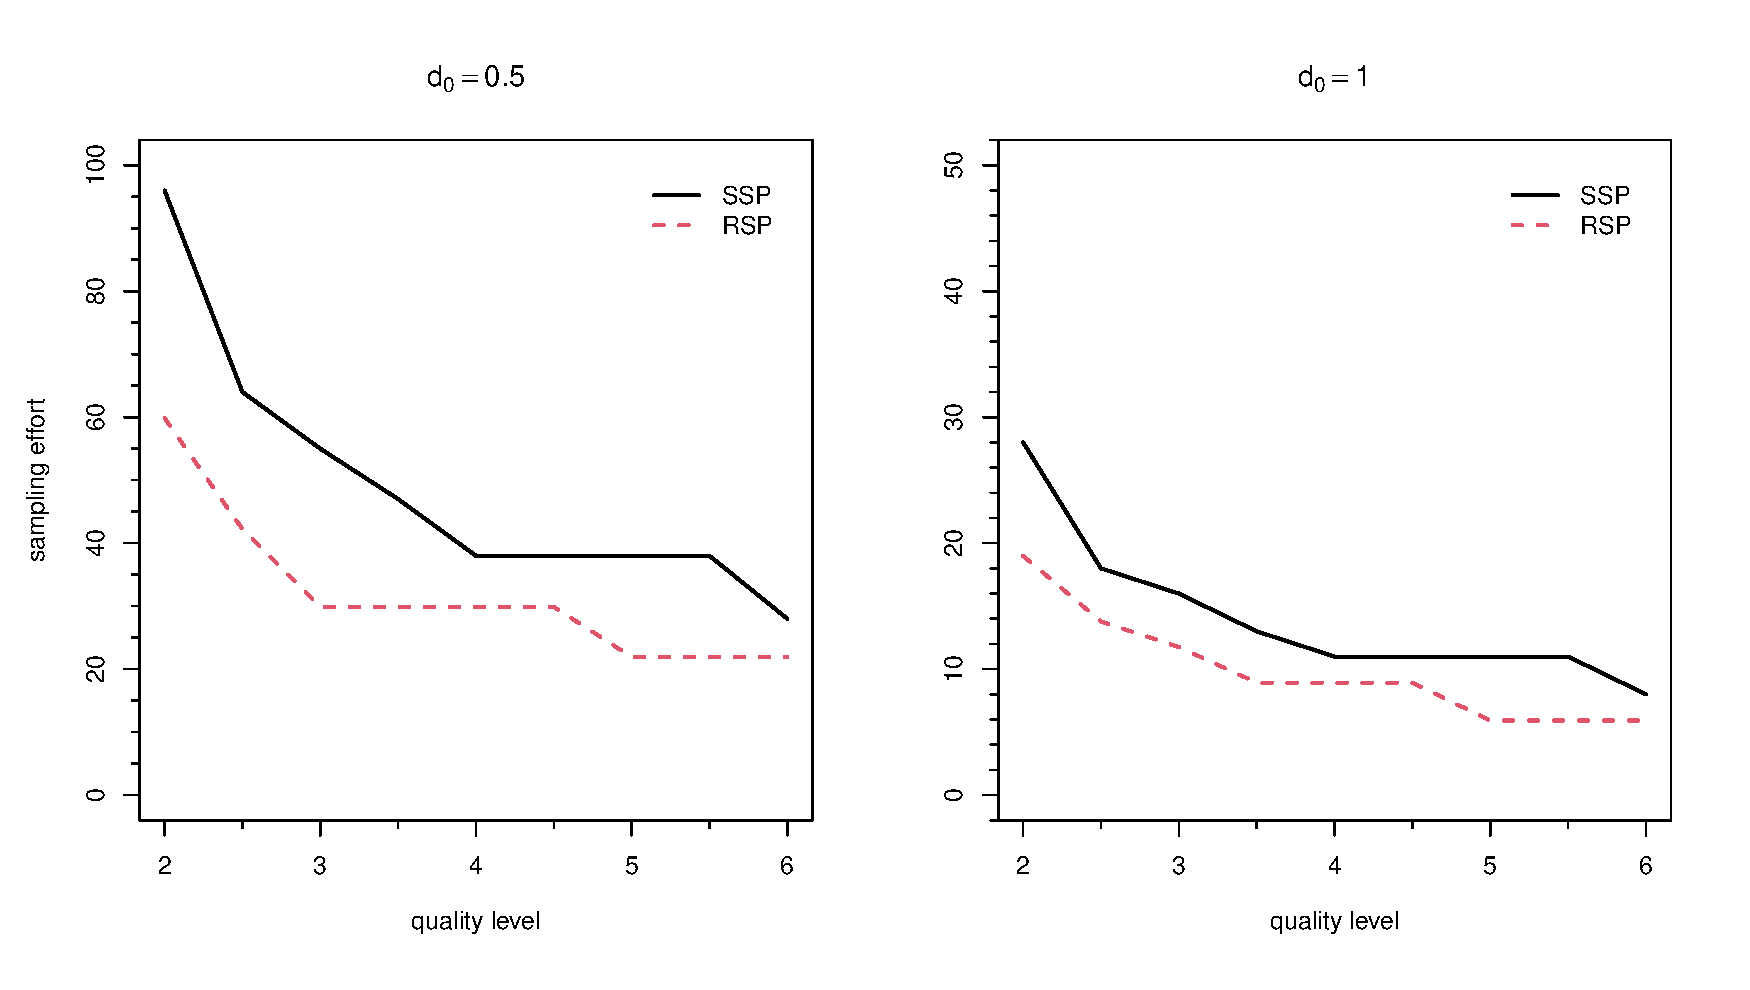
\includegraphics[width=15cm,height=8cm]{fig1.eps}\\
\vspace{-0.2cm}
\caption{\footnotesize{ASN curves for the SSP and the RSP versus the quality level $r_2$ when $\alpha=0.01, \beta=0.05, d_0=0.5,1.0$ and $\delta=1$.}}\label{fig1}
\end{center}
\end{figure}


\section{Real data application}
The results obtained in this paper are illustrated with application on a real data set. 
The following observations studied by \cite{Nelson}  are from an accelerated life test of 59 conductors
2.997, 4.137, 4.288, 4.531, 4.700, 4.706, 5.009, 5.381, 5.434, 5.459 5.589, 5.640,
5.807, 5.923, 6.033, 6.071, 6.087, 6.129, 6.352, 6.369 6.476, 6.492, 6.515, 6.522,
6.538, 6.545, 6.573, 6.725, 6.869, 6.923 6.948, 6.956, 6.958, 7.024, 7.224, 7.365,
7.398, 7.459, 7.489, 7.495 7.496, 7.543, 7.683, 7.937, 7.945, 7.974, 8.120, 8.336,
8.532, 8.591 8.687, 8.799, 9.218, 9.254, 9.289, 9.663, 10.092, 10.491, 11.038.
%
%
We consider some well-known distributions in order to illustrate the goodness of fit of the LR as follows:
\begin{itemize}
\item[1.]~Logistic-Exponential (LE) distribution with pdf:
\begin{eqnarray*}
f_{LE}(t)=\theta \delta e^{\theta t}\left(e^{\theta t}-1\right)^{\delta-1}\Bigl\{1+\left(e^{\theta t}-1\right)^{\delta}\Bigr\}^{-2},
~~t>0,~\delta>0,~\theta>0.
\end{eqnarray*}
%%
%%
\item[2.]~Generalized Exponential (GE) distribution with pdf:
\begin{eqnarray*}
f_{GE}(t)=\delta \theta e^{-\theta t}\left(1-e^{-\theta t}\right)^{\delta-1},~~t>0,~\delta>0,~\theta>0.
\end{eqnarray*}
%%%
%%%
\item[3.]~Exponential power (EP) distribution with pdf:
\begin{eqnarray*}
f_{EP}(t)=\delta \theta^{\delta} t^{\delta-1}e^{-(\theta t)^{\delta}}\exp\!\left\{1-e^{(\theta t)^{\delta}}\right\},~~t>0,~\delta>0,~\theta>0.
\end{eqnarray*}
\end{itemize}
%
%
The eligibility of data for the  LR distribution  was assessed using the Akaike information criterion (AIC), Bayesian information criterion (BIC), the log-likelihood (LL) function, Kolmogorov-Smirnov (K-S) statistic and p-value. Table \ref{tab03} displays the model fitting summary of the chosen data set. From Table \ref{tab03}, it is clear that  the  LR distribution is best fit for considered data set as compared to LE, GE and EP distributions.
%
\begin{table}
\centering
\caption{Distribution fit test results of considered data set.}\label{tab03}
\begin{tabular}{lccccccccccc}
\hline
\textbf{Model} &&& \textbf{-LL} && \textbf{AIC} && \textbf{BIC} && \textbf{KS} && \textbf{p-value} \\
\hline
LR     &&& 111.2049& & 226.4098 && 230.5649 && 0.0479 && 0.9983 \\
LE    &&& 111.5138 && 227.0276 && 231.1827 && 0.0492 &&0.9975 \\
GE     && & 114.9473 && 233.8946 && 238.0497 && 0.1042 &&0.5103 \\
EP      &&& 116.5015 && 237.0029 && 241.1580 && 0.1365 && 0.2021 \\
\hline
\end{tabular}
\end{table}
The maximum likelihood estimates of the  parameters are $\hat \delta=2.6968$ and $\hat\theta=0.0290$. 
 Using the fact $\mathcal{M}=[2\log2/\theta]^{0.5}$, the median life can be estimated as $\mathcal{M}_0=6.914$. Considering the termination ratio for this data set  as $d_0=1$, we  get the termination time $t=3.457$ minutes. Given $r_1=1, r_2=2$ and $(\alpha,\beta)=(0.01,0.05)$.
 Then, the optimal RSPs  are $(0,1,5)$ with corresponding ASN as 5.93.
The decision process can be stated as follows: 
\begin{itemize}
\item Step 1: Select a sample of size $n^{\star}=5$ from the submitted lot and put on test for  time $t=3.457$ minutes.
\item Step 2: If there is no failure before time $t=3.457$ minutes, accept the lot. If  there is more than  one  failure,  reject the lot and terminate the test. 
\item Step 3: If  there is one failure, i.e., $\mathcal{D}=1$, then go to step 1 and repeat the experiment.
\end{itemize}



\section*{Discussion and Conclusion}   
Time-censored repetitive sampling plans for \textit{LR} distribution are introduced in this paper. 
The \textit{LR} distribution is used to model the product time-to-failure.
In our situation, the proposed plans depend on the median lifetimes specified by the producer and the consumer, for given maximum admissible sampling risks. 
The \textit{RSP} that minimizes the ASN was derived by solving the corresponding integer nonlinear programming. From an inspection-effort perspective, the proposed RSPs outperform traditional SSPs. Traditional SSPs are simple but often require large sample sizes, resulting in high costs, especially for expensive or safety-critical products. RSPs typically reduce sample sizes. 



%\section*{Acknowledgments}   
%%%%%%%%%%%%%%%%%%%%%%%% References %%%%%%%%%%%%%%%%%%%%%%%%%%%%%

\begin{thebibliography}{9}


\bibitem[Chaudhary and Kumar(2020)]{Cha} Chaudhary A.K. and Kumar V. (2020), The logistic-Rayleigh distribution with properties and applications,
{\it International Journal of Statistics and Applied Mathematics}, 5(6), 12-19.

\bibitem[Jeyadurga and  Balamurali(2025)]{Jeya2025}Jeyadurga P. and   Balamurali S. (2025), Determination and economic design of repetitive group sampling plan under two parameter Lindley distribution, {\it Quality Technology and  Quantitative  Management}, 22(3), 553-576.


  
 \bibitem[Naghizadeh Qomi and Aslam(2026)]{NA2026}Naghizadeh Qomi M. and Aslam M. (2026), Developing optimal group acceptance sampling plans based on Weibull distribution with limited risks, {\it Journal of Applied Statistics}, 53(7), 1237-1252. 

\bibitem[Naghizadeh Qomi and Fern\'{a}ndez(2024)]{NF2024} Naghizadeh Qomi M. and  Fern\'{a}ndez A.J. (2024), Optimal double acceptance sampling plans based on truncated life tests for Tsallis q-exponential distributions, {\it Journal of Applied Statistics},  51(16), 3456-3467. 


\bibitem[Naghizadeh Qomi et al.(2026)]{NFC2026} Naghizadeh Qomi M. Fern\'{a}ndez A.J. and P\'{e}rez-Gonz\'{a}lez C.J. (2026), Optimal truncated repetitive sampling inspection plans under time-censoring based on type-I half-logistic Nadarajah-Haghighi distribution. {\it Proceedings of the Institution of Mechanical Engineers, Part O: Journal of Risk and Reliability}, 240(2), 527-539.


\bibitem[Naghizadeh Qomi and Mahdizadeh(2025)]{NM2025}Naghizadeh Qomi M. and Mahdizadeh Z. (2025), Optimal repetitive acceptance sampling inspection plans by attributes based on type I censoring using two-point and limited weighted methods,  {\it  Journal of Statistical Sciences}, 19(1), 227-246.


\bibitem[ Naghizadeh Qomi et al.(2025)]{NPGF2025} Naghizadeh Qomi M. Piadeh M.  P\'{e}rez-Gonz\'{a}lez C.J. and   Fern\'{a}ndez A.J. (2025), Optimal acceptance sampling plans based on generalized half-normal distribution under time-censoring with conventional and expected limited risks, {\it  Communications in Statistics-Simulation and Computation}, 1-20, doi: 10.1080/03610918.2025.2512380.


\bibitem[Nelson and Doganaksoy(2023)]{Nelson} Nelson W. and Doganaksoy N. (2023), Statistical analysis of life or strength data from specimens of various
sizes using the power-(log) normal model. {\it Recent Advances in Life Testing and Reliability} (pp. 377-408).



\bibitem[Sherman(1965)]{Sherman}  Sherman R.E. (1965), Design and evaluation of a repetitive group sampling plan, {\it Technometrics},  7, 11-21 .





\end{thebibliography}
 \end{document}

